\documentclass[10pt,a4paper,titlepage]{book}
\usepackage[utf8]{inputenc}
\usepackage{amsmath}
\usepackage{amsfonts}
\usepackage{amssymb}
\usepackage{graphicx}
\usepackage[colorlinks=true,linkcolor=blue]{hyperref}
\usepackage[left=2cm,right=2cm,top=2cm,bottom=2cm]{geometry}
\usepackage[font=small,labelfont=bf]{caption}
\usepackage{times}
\usepackage{subcaption}
\usepackage{parskip}
\usepackage{enumitem}
\usepackage{courier}
\usepackage[toc,page]{appendix}
\usepackage{listings}
\setlist{noitemsep}


\begin{document}

\begin{titlepage}
	\centering
	{\scshape\LARGE Spatial Transcriptomics Viewer v0.6.3 User Manual\par}
	\vspace{1cm}
	{\Large Jose Fernandez Navarro\par}
	\vspace{1cm}
	{\today\par}

\end{titlepage}

\pagenumbering{Roman}

\subsection*{Preface}
The Spatial Transcriptomics viewer (ST viewer) is a desktop application that allows users to securely access and visualize spatially distributed gene expression profile data with their respective tissue image. At the same time it allows users to analyze the data directly, or export it for their own analyses. The application can obtain the data from a secured server (configuration files will need to be updated for this) and/or from local files.


For installation instructions, please see the README.md file. This file describes the install instructions on Windows, OSX and Linux.

{\textbf{Licensing}}

This is open source software under the MIT license.
Read LICENSE for more information about the licensing terms.

{\textbf{Contact}}

Please report bugs, feedback, questions and errors to:\\
Jose Fernandez Navarro (\href{mailto:jose.fernandez.navarro@scilifelab.se}{jose.fernandez.navarro@scilifelab.se}) or\\
Alexander Stuckey (\href{mailto:alexander.stuckey@scilifelab.se}{alexander.stuckey@scilifelab.se})



\tableofcontents
\raggedbottom
\clearpage
\listoffigures
\pagenumbering{arabic}

\chapter{Spatial Transcriptomics Technology}
\label{ch:st_tech}
\section{What is Spatial Transcriptomics}
Spatial Transcriptomics is a method that allows  visualization and quantitative analysis of the transcriptome in individual tissue sections. By placing histological sections on glass slides with arrayed oligonucleotides containing positional barcodes, it is possible to generate high quality cDNA libraries with precise positional information for RNA-seq. This provides transcriptoms data in a versitile format for bioinformatic analyses of gene expression within the tissue context, valuable on both research and diagnostics.

\section{What is a Spatial Transcriptomics dataset}
A Spatial Transcriptomics dataset is a tab seperated text file containing counts for each gene at each position on the array (table \ref{tab:st_dataset}).

\begin{table}[h]
\begin{center}
\caption{A general example of a Spatial Transcriptomics dataset file.}
\begin{tabular}{c | cccc}
 & Gene A & Gene B & Gene C & ... \\ \hline
1x1 & 12 & 0 & 27 & ... \\
2x1 & 64 & 62 & 63 & ... \\
3x1 & 375 & 43 & 0 & ... \\
... & ... & ... & ... & ... \\
\end{tabular}
\label{tab:st_dataset}
\end{center}
\end{table}

This dataset is generated from the ST\_Pipeline (obtainable from GitHub,\\ \url{https://github.com/SpatialTranscriptomicsResearch/st_pipeline}).\\ However, although the ST\_Pipeline outputs a tab seperated file, the current version of the ST\_viewer (v0.6.3) only supports data in the JSON file format. To convert from \texttt{.tsv} files to \texttt{.json} files, the python script \texttt{matrix\_to\_json.py} can be used. It can also be obtained from GitHub (\url{https://github.com/SpatialTranscriptomicsResearch/st_analysis}), in the \texttt{scripts} folder. Further releases of the viewer will be able to read \texttt{.tsv} files directly, eliminating the need to convert to \texttt{.json} first.

\chapter{Installing and Running the Spatial Transcriptomics Viewer}
\section{Installing the viewer}
The viewer can be installed for Windows, MacOSX and UNIX PCs. Build instructions can be found on the spatial transcriptomics \href{https://github.com/SpatialTranscriptomicsResearch/st_viewer}{GitHub page}. The same instructions can also be found in the README.md file in the GitHub repository. They can also be found in Appendix \ref{Appendix A} in this manual.

\section{Running the Viewer}
\subsection*{MacOSX}
To run the viewer on OSX, simply double click the app icon that you built in the previous step. It can be found in \texttt{/path/to/build}. For ease of use, the app can be copied to the applications folder. It can then be opened using spotlight search (press command + space, then type stviewer).

\subsection*{Windows}
To run the viewer in Windows, double click the desktop icon (if created during install), click the start menu shortcut (\texttt{Start $\rightarrow$ Programs $\rightarrow$ STViewer}, if created during install) or navigate to the folder where the viewer was installed and double click the icon.

\subsection*{UNIX}
To tun the viewer in UNIX, open a terminal and type \texttt{/path/to/bin/STViewer}. Alternatively, you can add the path to the binary to the system PATH variable, create a symlink to the binary in \texttt{/usr/bin} or \texttt{\$HOME/bin} (if it exists and is in your \$PATH) or move the binary to \texttt{/usr/bin} or \texttt{/\$HOME/bin}. To add a directory to your \$PATH variable, open the \texttt{.bashrc} file (or equivalent e.g. \texttt{.zshrc}) found in your \$HOME directory with your favourite text editor. At the end of the file add the following line: \texttt{export PATH="\$PATH:/path/to/directory/"}. Then, close your terminal or enter \texttt{source .bashrc} (or equivalent). The \texttt{.bashrc} file is a hidden file, so it is not normally visible in the directory. The easiest was to edit the file is to open a terminal and type \texttt{gedit .bashrc}.

\chapter{General Overview}
\section{Online Database}
The online mode is only supported if the user sets up their own ST server and configures the database and ST API/ADMIN correctly. Instructions for how to do this can be found on GitHub at the following address \url{https://github.com/SpatialTranscriptomicsResearch/st_api}. How to use the viewer in offline mode can be found in chapter \ref{sec:local_data}.
\section{User Interface}
 When running the spatial transcriptomics viewer for the first time, you will be presented with an interface as shown in figure \ref{fig:default_view}. If the viewer has been configured to access datasets through the ST API then the login window will be shown, otherwise it will not be shown.
\begin{figure}[h]
	\centering
	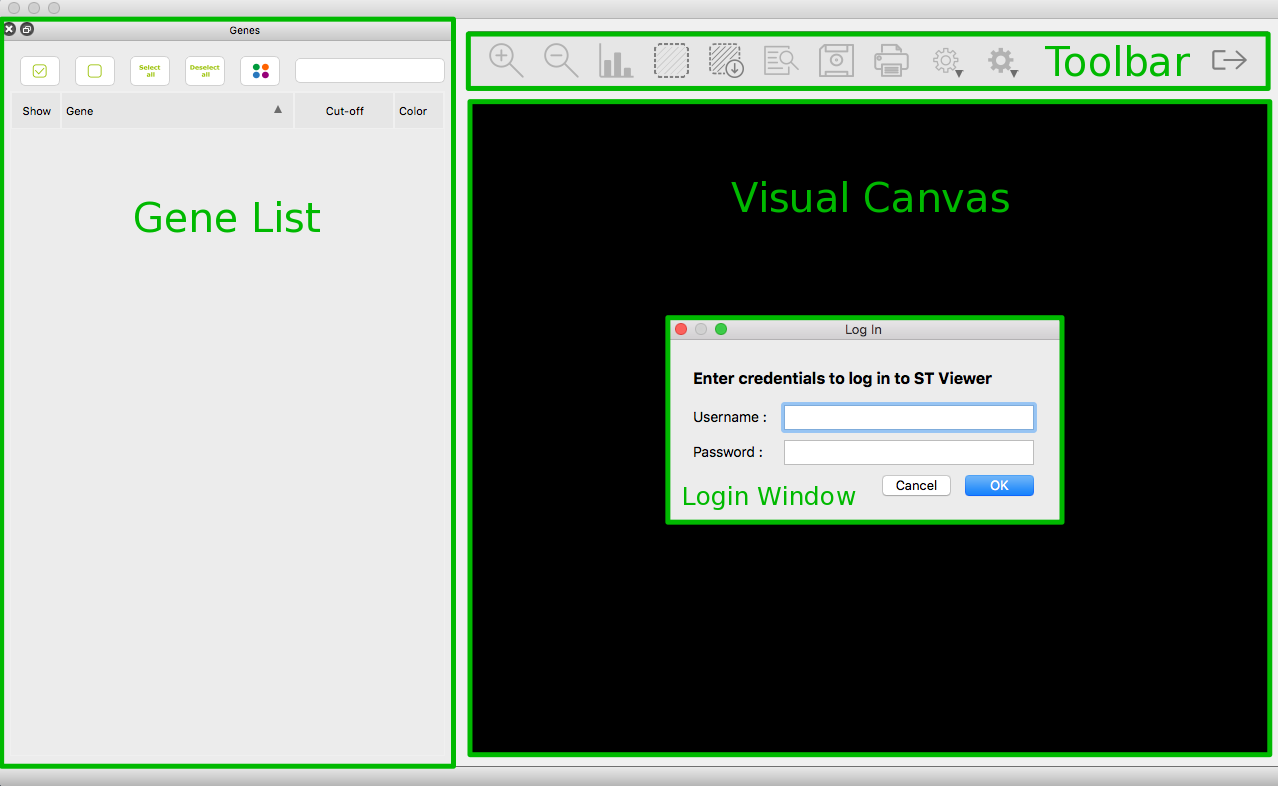
\includegraphics[width=0.8\linewidth]{./Pictures/default_logged_out_labelled}
	\caption[The spatial transcriptomics viewer default interface]{The default interface presented when the ST viewer is run for the first time. The elements present are the gene list window on the left, the toolbar in the top right, the visual canvas on the right, and optionally the log in window (if the viewer is configured to access datasets through the ST API).}
	\label{fig:default_view}

\end{figure}

The menu bar has two options, \texttt{File} and \texttt{Views}. In the \texttt{File} menu you are able to view information about the viewer, as well as clear the local cache (doing so will force any datasets to be re-downloaded or re-imported). This is useful when changes have been made to the external datasets. The \texttt{Views} menu toggles the display of the \texttt{datasets}, \texttt{selections} and \texttt{genes} windows. It also contains the logout toggle, if you can connect to an online database.

Once you have logged in (if applicable), your user name will be displayed in the toolbar, as shown in figure \ref{fig:user_name}.
\begin{figure}[h]
	\centering
	
\includegraphics[width=0.8\linewidth]{./Pictures/logged_in}
	\caption{Toolbar showing username after logging in.}
	\label{fig:user_name}
\end{figure}

There are two other main windows in the ST viewer, datasets and selections. They can both be accessed from the views menu by clicking \texttt{views} $\rightarrow$ \texttt{datasets} and \texttt{views} $\rightarrow$ \texttt{selections}.
The datasets window shows all the datasets that you have access to. There is a search box that can be used to find a keyword in the dataset names to narrow down the list of datasets (see figure \ref{fig:datasets_view}). There are five buttons to the right of the dataset search box (labelled 1 --- 5). They are:
\begin{enumerate}
\item Import dataset from file (local file on your computer)
\item Open selected dataset (for datasets stored in the database)
\item Edit selected dataset (change name, add comments)
\item Delete selected dataset
\item Refresh list of datasets
\end{enumerate}

The datasets displayed in the dataset view can also be sorted by each column (e.g. name or species).
\begin{figure}[h]
	\centering
	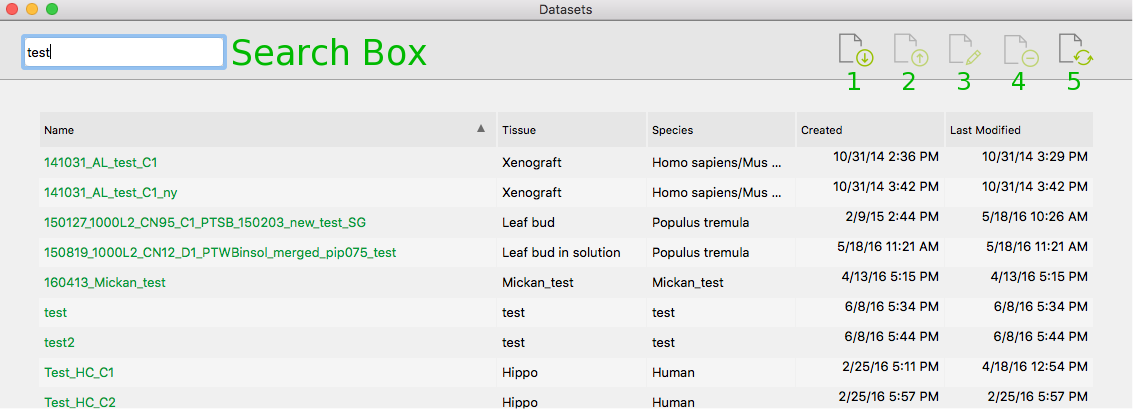
\includegraphics[width=0.8\linewidth]{./Pictures/datasets}
	\caption[Datasets view.]{Datasets view. The search box is being used to display only the datasets that contain the word "test" in their name.}
	\label{fig:datasets_view}
\end{figure}

The selection view will be discussed further in chapter \ref{ch:selection}.

{ \textbf Note:} 
Each dataset is associated with a substantial amount of data, which will be accessed after a dataset has been selected and opened. As such the transition between the views might require a few moments. It is worth noting that the data is cached, which implies that once it is downloaded, the next time the same dataset will open much quicker. This does not apply if the dataset is updated in the cloud in the meantime.

Opening a new dataset while a previous dataset is open can be done in the same manner as opening a dataset for the first time. Note that when this is done the visualisation settings are set back to the defaults.

When the dataset is loaded, the visual canvas will display with a picture of the tissue. This picture can be zoomed (using the scroll-wheel on the mouse) and panned by clicking and holding left click while dragging the mouse around.

When a dataset is loaded, the gene list will populate with the list of all genes that are associated with the current dataset, and the visual canvas will display the image of the tissue section (see figure \ref{fig:default_loaded_data}). 
\begin{figure}[h]
	\centering
	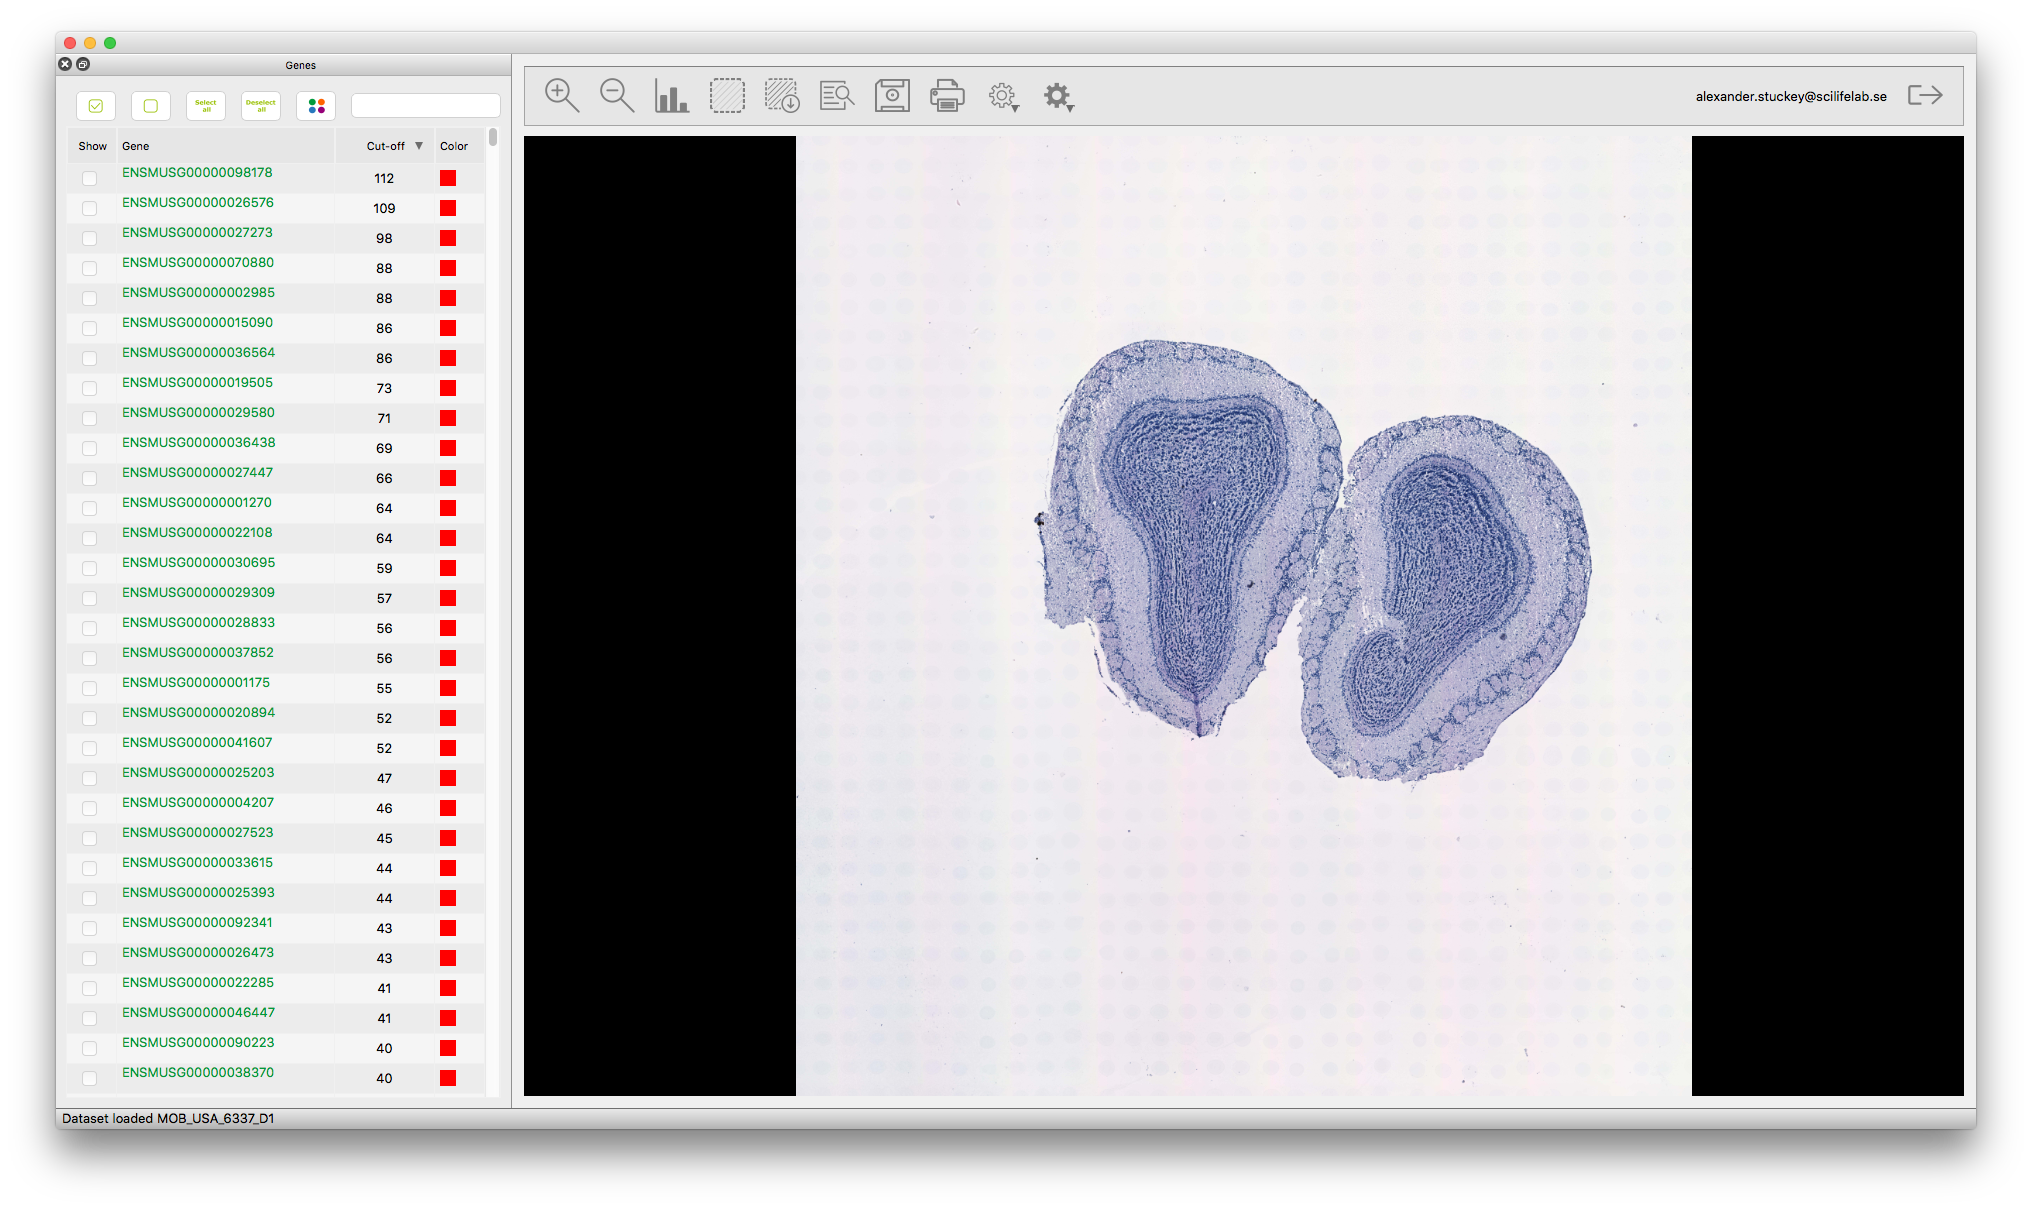
\includegraphics[width=0.8\linewidth]{./Pictures/default_dataset_loaded}
	\caption[Default view after loading a dataset]{The default view after loading a dataset. The gene list is populated by all the genes in the data, and an image of the tissue section is presented on the visual canvas.}
	\label{fig:default_loaded_data}
\end{figure}

The gene list is headed by five buttons and a text box. The buttons are, in order:
\begin{enumerate}
\item	Show selected
\item	Hide selected
\item	Select all
\item	Deselect all
\item	Set colour
\item	Search box
\end{enumerate}

The text box enables you to search the list of genes for genes that are of interest. Shown genes are marked with a checkmark in the box to the left of the gene name / ensemble ID. Selected genes have their names highlighted in orange instead of green, and have a darker grey background. Note that shown genes and selected genes may differ (as seen in figure \ref{fig:gene_list}). The colour column allows you to choose custom colours for single genes or groups of genes, in order to increase visual clarity. The gene list can also be sorted by gene name and cut-off value.

The cut-off value is only important (and only makes sense) if all of the positions on the array are being used. If the st\_data file has been edited so that only the positions that are under the tissue are being used, the cut-off should be disregarded. Additionally, the option \texttt{Individual gene cut-off} in the \texttt{Gene display configuration} menu should be disabled.

\begin{figure}[h]
	\centering
	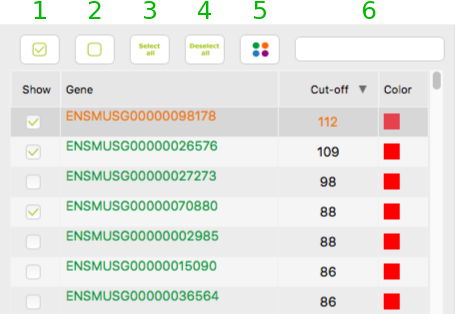
\includegraphics[scale=0.7]{./Pictures/gene_list}
	\caption[Gene List]{Gene list for the current dataset, sorted by cut-off value.}
	\label{fig:gene_list}
\end{figure}

When a dataset is loaded into the viewer the buttons above the visual canvas become active (figure \ref{fig:toolbar_data_loaded}). The buttons on the toolbar are:
\begin{enumerate}
\item	Zoom in
\item	Zoom out
\item	Feature distribution histograms
\item	Selection mode toggle
\item	Create selection object
\item	Feature selection by regular expression
\item	Save a picture of the visual canvas
\item	Print a picture of the visual canvas
\item	Gene display configuration
\item	Visual canvas options
\item	Logout button
\end{enumerate}

\begin{figure}[h]
	\centering
	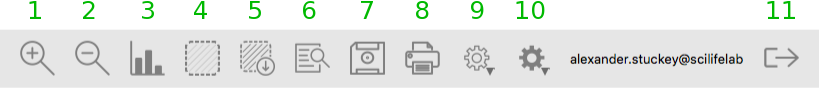
\includegraphics[width=0.8\linewidth]{./Pictures/toolbar_data_loaded}
	\caption{The toolbar when a dataset is loaded.}
	\label{fig:toolbar_data_loaded}
\end{figure}

The visual canvas option menu allows us to display a legend for the overall expression values for each spot (useful in heatmap mode). It can also be used to toggle display of the tissue image (and any secondary image) off and on again.

The gene display configuration is shown in figure \ref{fig:gene_display_config}. From top to bottom, the options are:\\
\textbf{Show Grid} toggles the display of the original array and its border simplified to $5*5$ features per square.\\
\textbf{Show Genes} toggles the display of the currently selected genes.\\
\textbf{Choose Colour Grid} opens a menu to change the colour of the displayed array grid.\\

\section{Gene Display Modes}

\begin{figure}[h]
	\centering
	\begin{subfigure}{0.3\linewidth}
		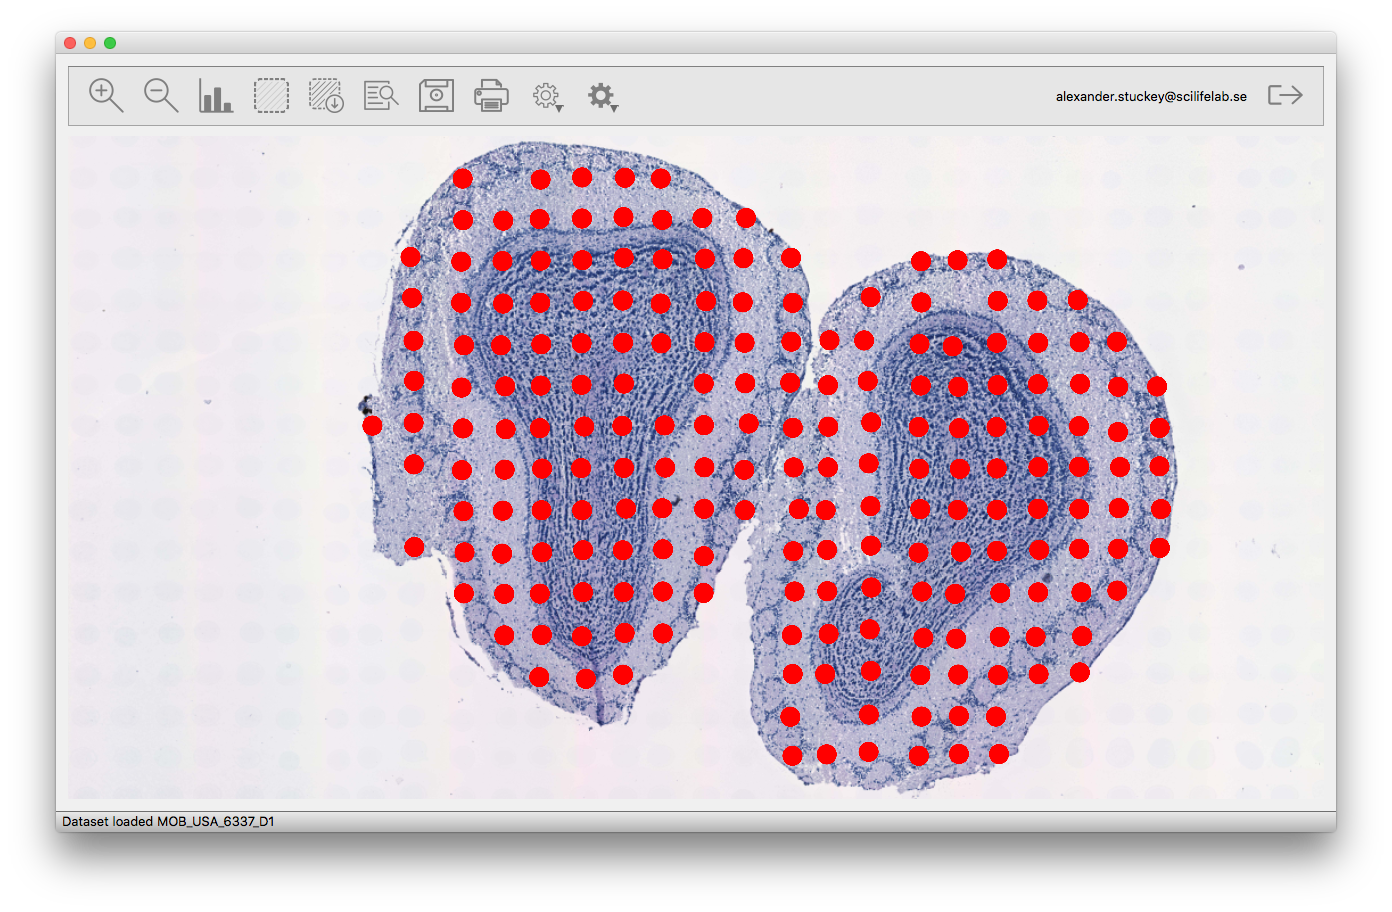
\includegraphics[width=\linewidth]{./Pictures/vc_normal}
		\caption{Visual canvas in normal mode.}
		\label{fig:vc_normal}
	\end{subfigure}
	\begin{subfigure}{0.3\linewidth}
		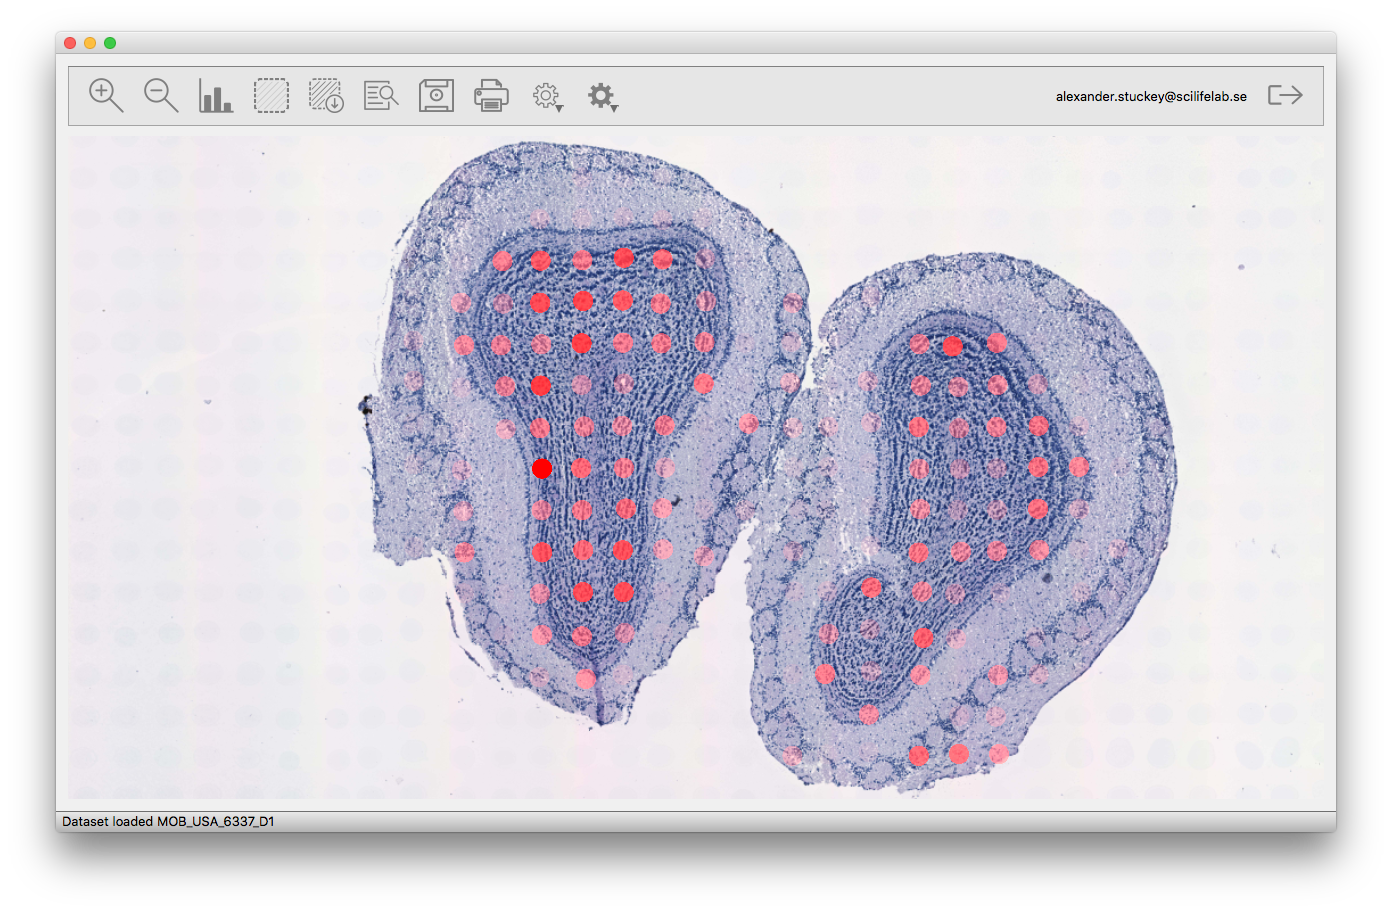
\includegraphics[width=\linewidth]{./Pictures/vc_dynamic}
		\caption{Visual canvas in dynamic mode.}
		\label{fig:vc_dynamic}
	\end{subfigure}
	\begin{subfigure}{0.3\linewidth}
		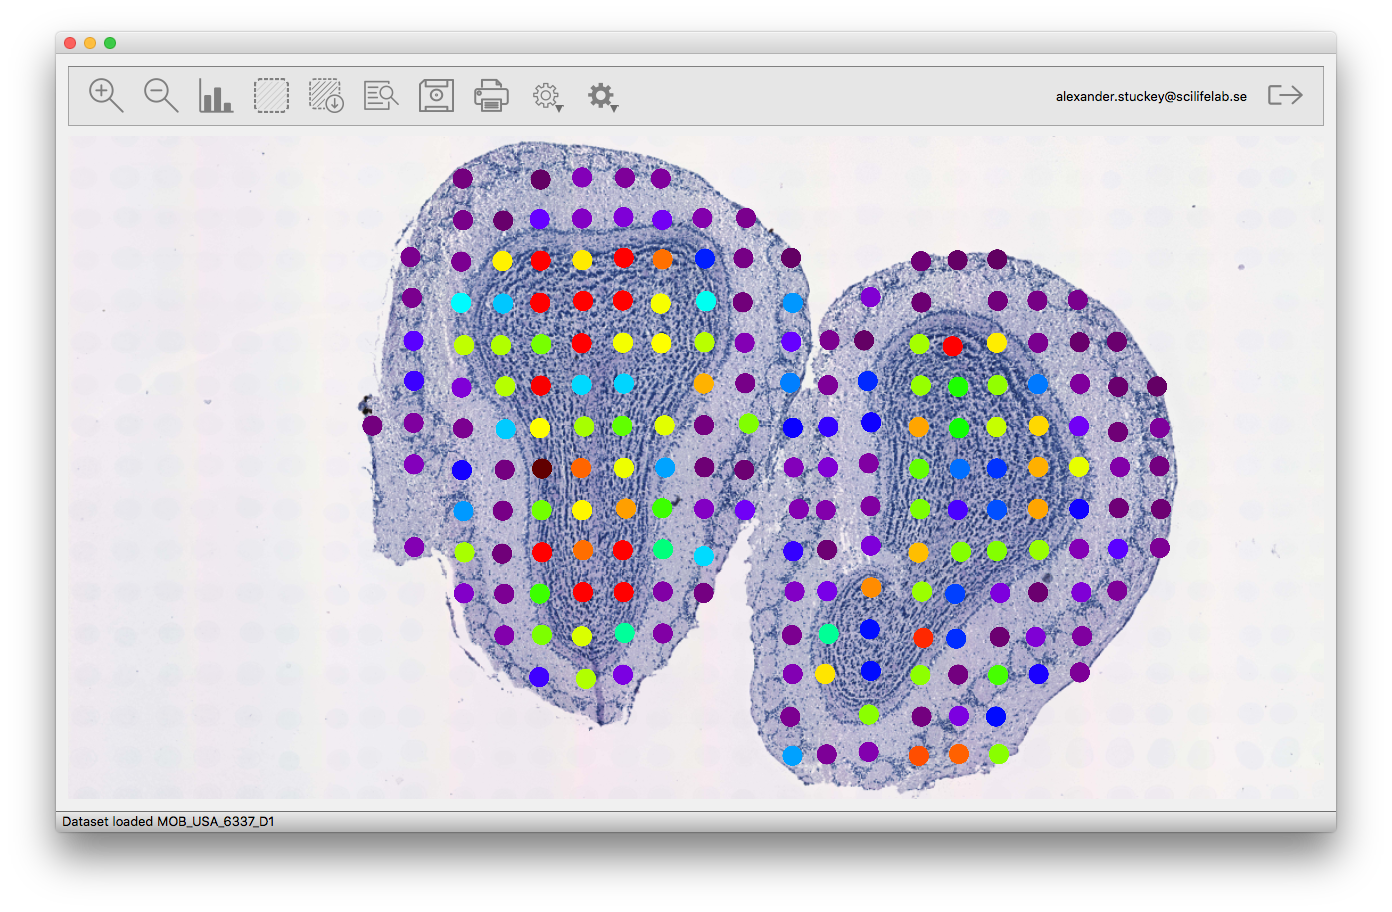
\includegraphics[width=\linewidth]{./Pictures/vc_heatmap}
		\caption{Visual canvas in heatmap mode}
		\label{fig:vc_heatmap}
	\end{subfigure}
	\caption[The visual canvas of the ST viewer in each map mode.]{The visual canvas of the ST viewer in the normal, dynamic and heatmap map modes. All genes are selected in these images, with all colours set to the defaults.}
\end{figure}

In \textbf{Normal Mode} (figure \ref{fig:vc_normal}) the selected genes in each feature are treated independently. When multiple genes are selected, the final colour of the feature will be a mix of the different colours of the selected genes. In normal mode, the threshold setting treats the genes in each feature separately. Therefore, the threshold can hide some of the selected genes in a feature, or even all the genes in a feature. In all cases, the final colour of the feature will be adjusted accordingly.

In \textbf{Dynamic Range Mode} (figure \ref{fig:vc_dynamic}) the selected genes in a feature are all treated as one unit (as opposed to normal mode). This means that each feature is treated as a single unit where the level of expression is determined by the combination of all the genes selected in the feature. The final expression is normalised and the alpha channel (the brightness) of the feature is adjusted according  to the normalised final expression of the feature. This way, users can get an idea of the total expression level of a feature compared to all other features. The colour of each feature will be computed in the same way as in the normal mode (it combines the colours of the genes in each feature).
The threshold in dynamic mode affects features as a whole, instead of gene-by-gene as in normal mode. When the threshold is changed the intensity for all the features is re-calculated, as the normalisation factor might have changed.

\textbf{Heatmap Mode} (figure \ref{fig:vc_heatmap}) treats genes in a feature in the same manner as the dynamic range mode. Instead of adjusting the brightness of the colour, a new colour is computed for the feature representing the overall level of expression. The low frequencies are blue and represent a low hit count, while the high frequencies are red and represent a high hit count. The heatmap spectrum and threshold levels can be seen on the legend, when the legend is enabled.
The threshold works the same way as in dynamic range mode, when the threshold is changed the colour range and colour of features will be recalculated.

The individual gene cut-off is used in cases where the ST\_data file contains information for every spot, not just the spots that are under the tissue. In this case, the viewer calculates a cut-off for each gene where expression values under the cut-off are assumed to be outside of the tissue and removed from the display. Expression values that are higher than the cut-off value are assumed to be under the tissue and retained. Leaving this setting on when there is only data for spots under the tissue can result in odd behaviour, and masking of much informative data. It is recommended to disable this setting when the dataset has been edited to remove all spots that are not under the tissue.

The opacity, size and shape parameters change the display of the features on the visual map mode.

\begin{figure}[h]
	\centering
	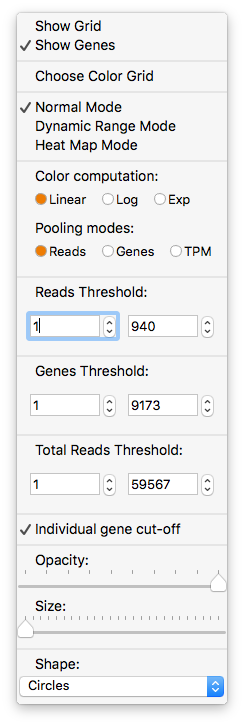
\includegraphics[scale=0.5]{./Pictures/menu_1}
	\caption{Gene display configuration}
	\label{fig:gene_display_config}
\end{figure}

\clearpage

\section{Importing a local dataset}
\label{sec:local_data}
To import a dataset locally, click \texttt{Views $\rightarrow$ Datasets}, then click \texttt{Import Dataset}. This brings up the import window (figure \ref{fig:import_local_dataset}).

\begin{figure}[h]
	\centering
	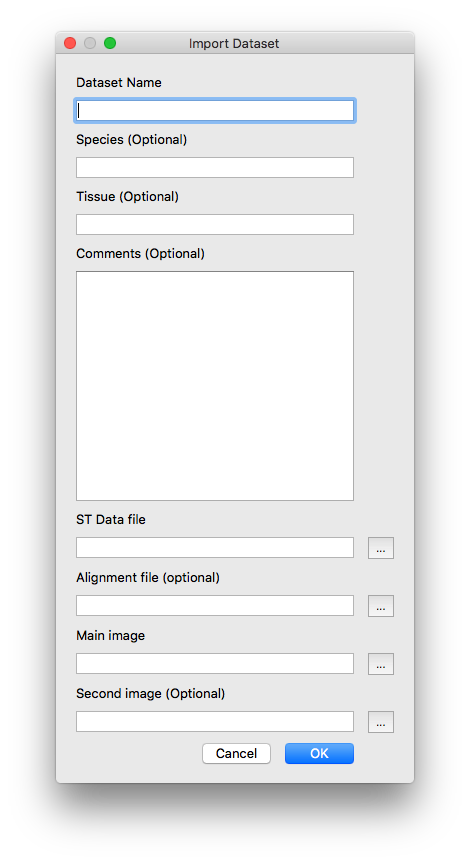
\includegraphics[scale=0.5]{./Pictures/import_dataset}
	\caption{The local dataset import window.}
	\label{fig:import_local_dataset}
\end{figure}

To import a dataset, you need to supply the information for each field. It is recommended to fill in each field (except for the second image field) so that it is easy to see what the dataset contains. The ST data file is the \texttt{.json} file obtained after running the st pipeline and converting the resulting \texttt{.tsv} file to \texttt{.json} format using the python script \texttt{matrix\_to\_json.py} described in chapter \ref{ch:st_tech}. The main image is the H\&E stained image of the tissue. 

The alignment file is used to convert between the array coordinates in the st\_data file (e.g. 1x2, 23x13) to exact pixel coordinates in the H\&E stained image. Doing so allows spots to be displayed in the correct position in the tissue image. The alignment matrix is in the following format:

\begin{table}[h]
\begin{center}
\caption{General alignment matrix format.}
\begin{tabular}{ccc}
scaling x & 0 & offset x \\
0 & scaling y & offset y \\
0 & 0 & 1 \\
\end{tabular}
\label{tab:align_matrix_format}
\end{center}
\end{table}

The scaling factor for x is the width of the image (in pixels) divided by the number of spots in one row (32). The scaling factor for y is the height of the image (in pixels) divided by the number of spots in one column (34). These numbers should be entered to one decimal place. An example off an scaling for x and y would be 294.2, 296.3. The offset describes how far from the top left corner of the image the center of the first spot is located. This value is the same as the scaling values, but negative. Examples of the offset using the same scaling values as before would be -294.2, -296.3. This means that we need to move 294.2 pixels right and 296.3 pixels down from the top left corner of the image to find the center of the first spot.

The alignment matrix that is needed for the viewer is a single tab seperated line of nine values. These can be obtained from the alignment matrix previously calculated. It has the following format:
\begin{table}[h]
\begin{center}
\caption{General alignment file form for the ST viewer.}
\begin{tabular}{*{9}{c}}
scaling x & 0 & 0 & 0 & scaling y & 0 & offset x & offset y & 1 \\
\end{tabular}
\label{tab:st_viewer_alignment}
\end{center}
\end{table}

Using the example numbers from earlier, the final alignment matrix example would be:

\begin{table}[h]
\begin{center}
\caption{An example of an alignment file for the ST viewer.}
\begin{tabular}{*{9}{c}}
294.2 & 0 & 0 & 0 & 296.3 & 0 & -294.2 & -296.3 & 1 \\
\end{tabular}
\label{tab:st_viewer_alignment_example}
\end{center}
\end{table}

It is important that the alignment file is written in a plain text editor and saved as a \texttt{.txt} file. Other editors and other file types can often insert invisible meta-characters into the file that will cause the viewer to crash. Nano, a terminal based text editor available on most Unix systems, is a good choice for writing alignment files. On Windows, notepad or notepad++ would be good alternatives.

All the different views are undockable from the main ST viewer window and can be shown at the same time.

\chapter{Using the Viewer}
\label{ch:selection}

\section{Selection Mode}
Selection mode is toggled using button 4 in \ref{fig:toolbar_data_loaded}. When selection mode is enabled the user is able to select features on the canvas by clicking and dragging a box on the visual canvas (figure \ref{fig:default_selection}). The user can select disjointed areas by holding down shift while selecting an area (figure \ref{fig:double_selection}). Areas can also be removed from the selection by either shift $+$ control (Windows and Linux) or shift $+$ command on Mac (figure \ref{fig:selective_selection}).

In addition to selecting via clicking and dragging on the visual canvas, users can also select genes via regular expressions (button 6 in figure \ref{fig:toolbar_data_loaded}). Regular expressions provide the user with a powerful means to select specific genes by matching the gene names against a specific string pattern. The regular expression syntax is modeled after the Perl regular expressions.
In addition the selection dialog provides three options; to include ambiguous genes, to select non-visible genes, and to make the regular expression case sensitive.
By default the regular expression selection excludes ambiguous genes and ignores case differences.


\begin{figure}[h]
	\centering
	\begin{subfigure}{0.3\linewidth}
		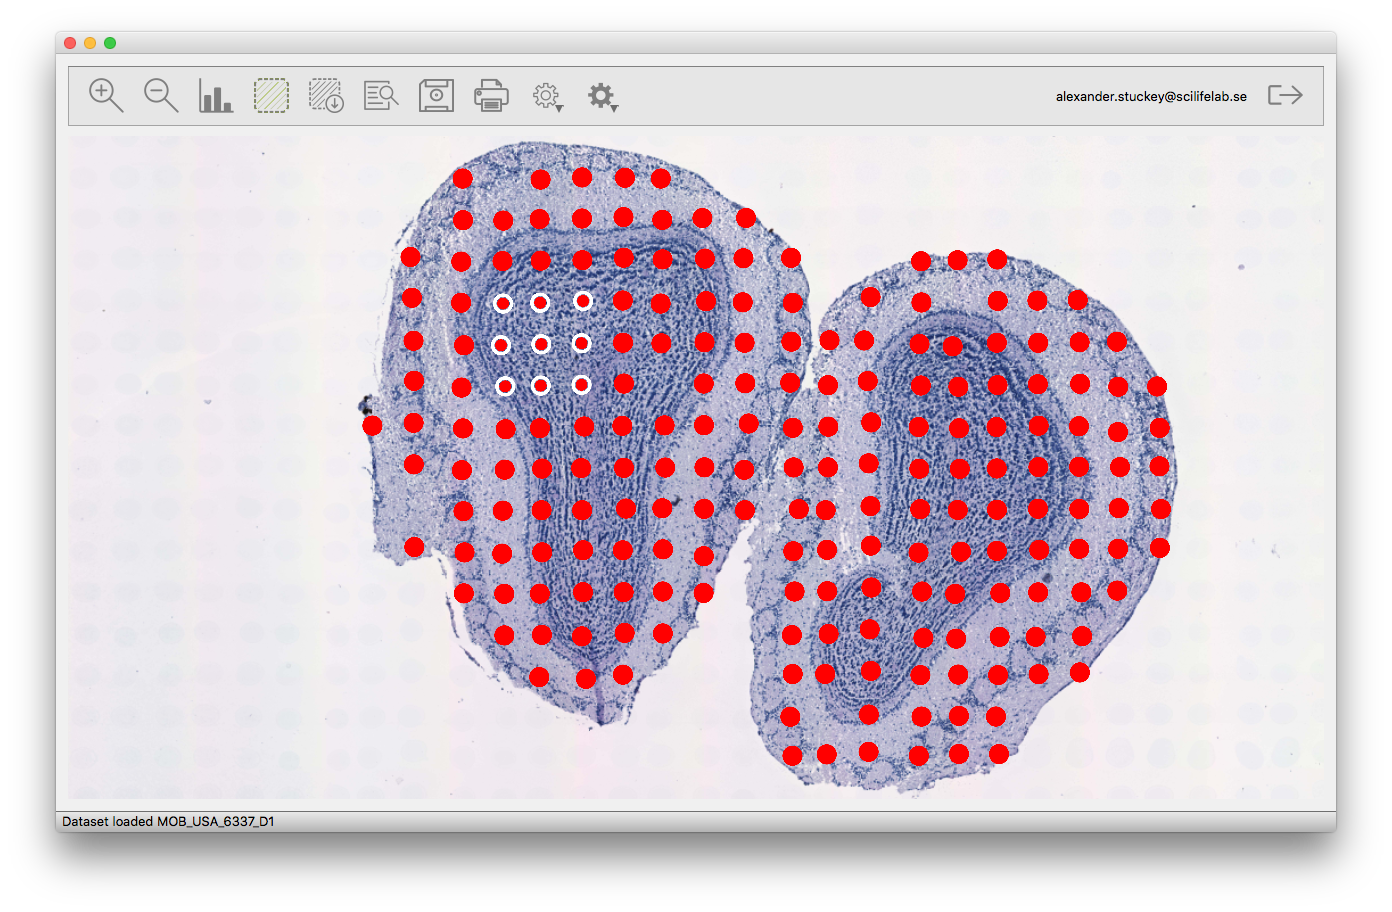
\includegraphics[width=\linewidth]{./Pictures/default_selection}
		\caption{Visual canvas with some features selected.}
		\label{fig:default_selection}
	\end{subfigure}
	\begin{subfigure}{0.3\linewidth}
		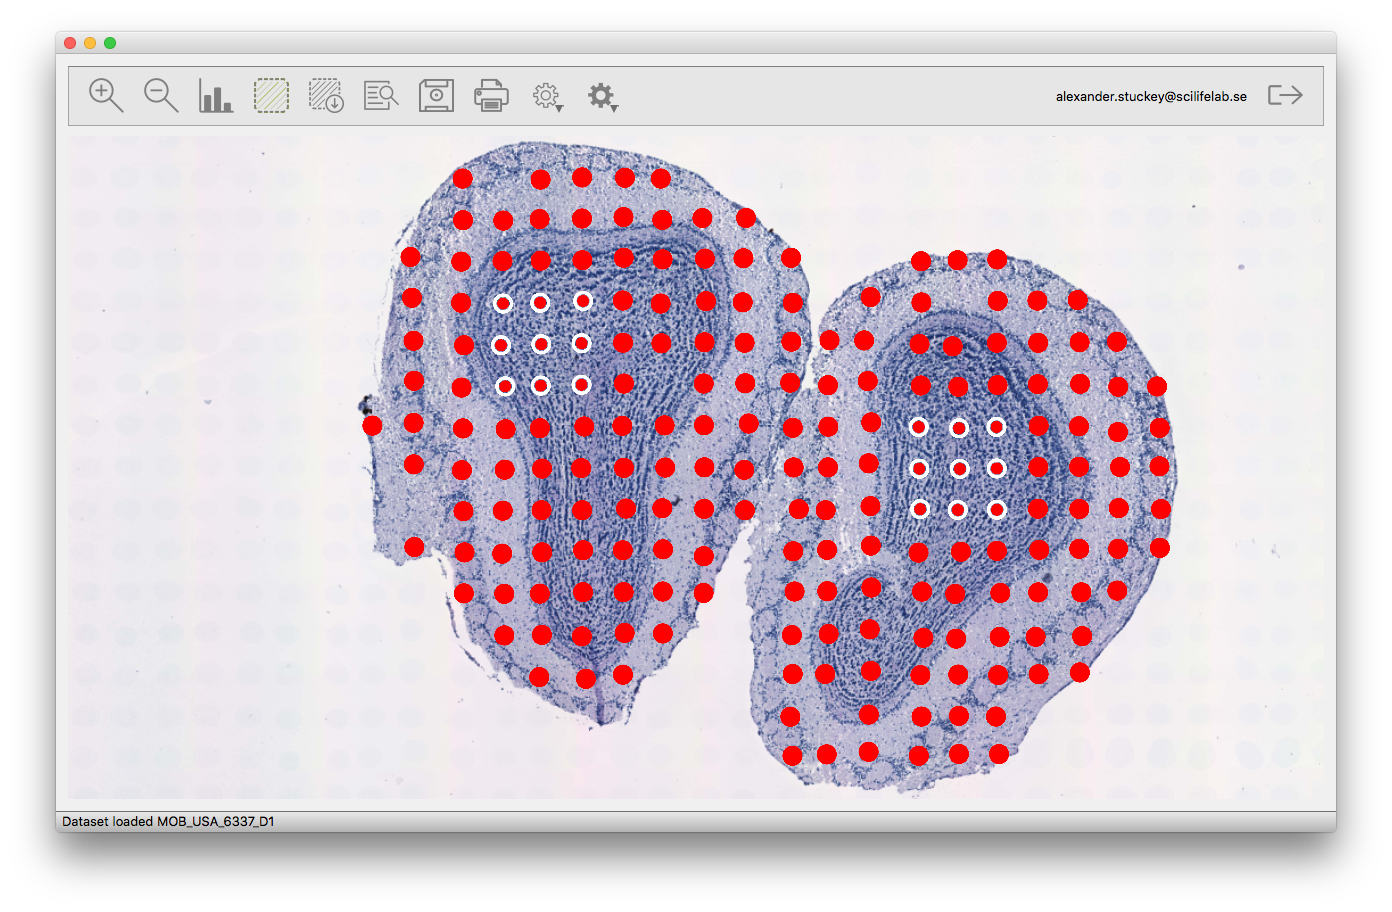
\includegraphics[width=\linewidth]{./Pictures/double_selection}
		\caption{Visual canvas with two disjointed regions of features selected.}
		\label{fig:double_selection}
	\end{subfigure}
	\begin{subfigure}{0.3\linewidth}
		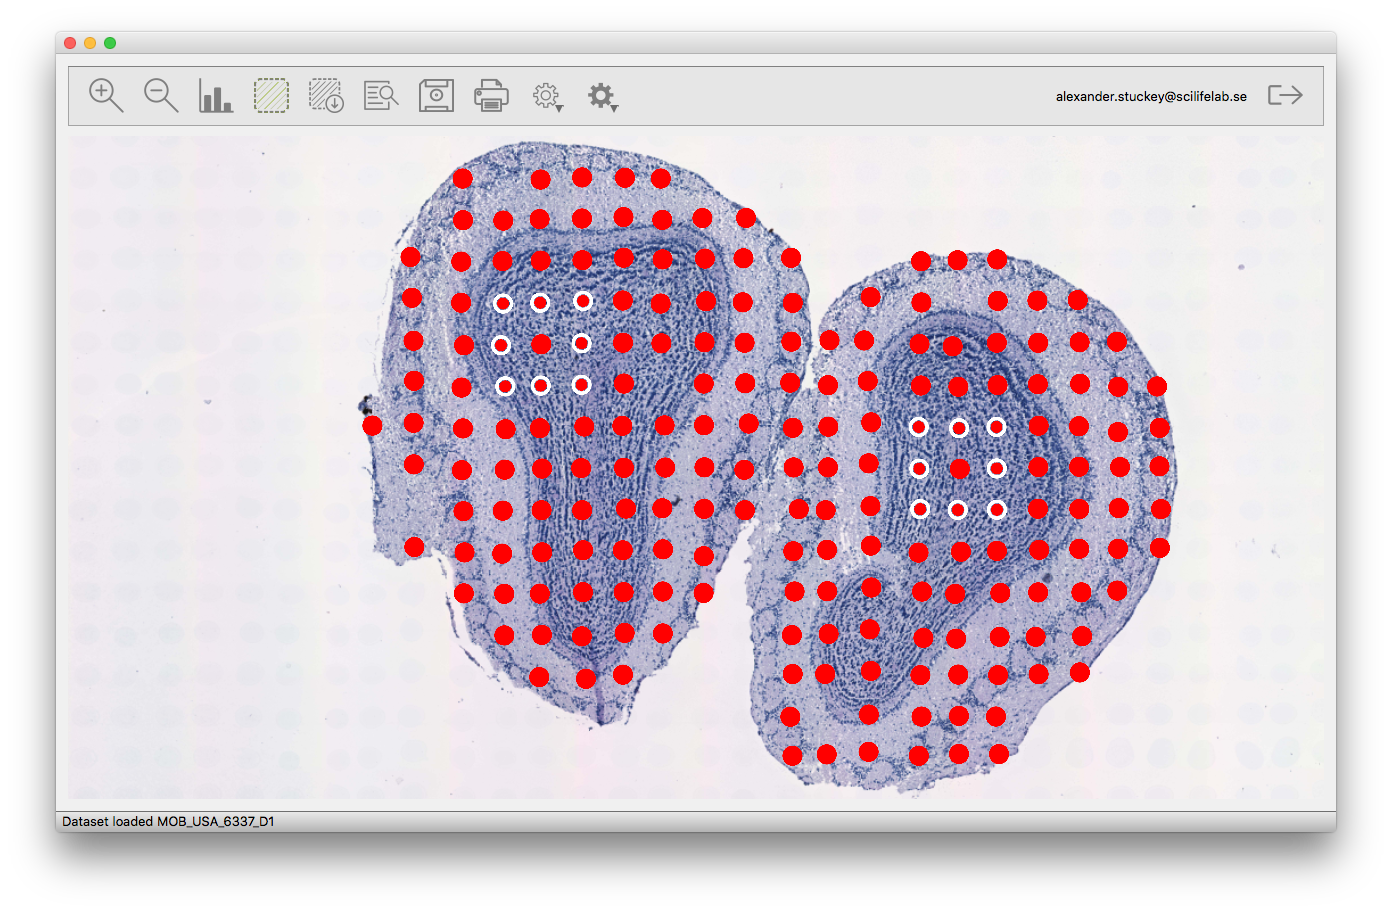
\includegraphics[width=\linewidth]{./Pictures/selective_selection}
		\caption{Visual canvas with two disjointed regions of features selected, with some interior features de-selected}
		\label{fig:selective_selection}
	\end{subfigure}
	\caption[The visual canvas of the ST viewer showing different selection types.]{The visual canvas of the ST viewer showing the different ways of selecting features.}
\end{figure}

When the desired features are selected, the user can create a selection object by clicking button 5 in \ref{fig:toolbar_data_loaded}. The selections can then be viewed by clicking on views $\rightarrow$ selection. This brings up the selection window (figure \ref{fig:selection_menu}).

\begin{figure}[h!]
	\centering
	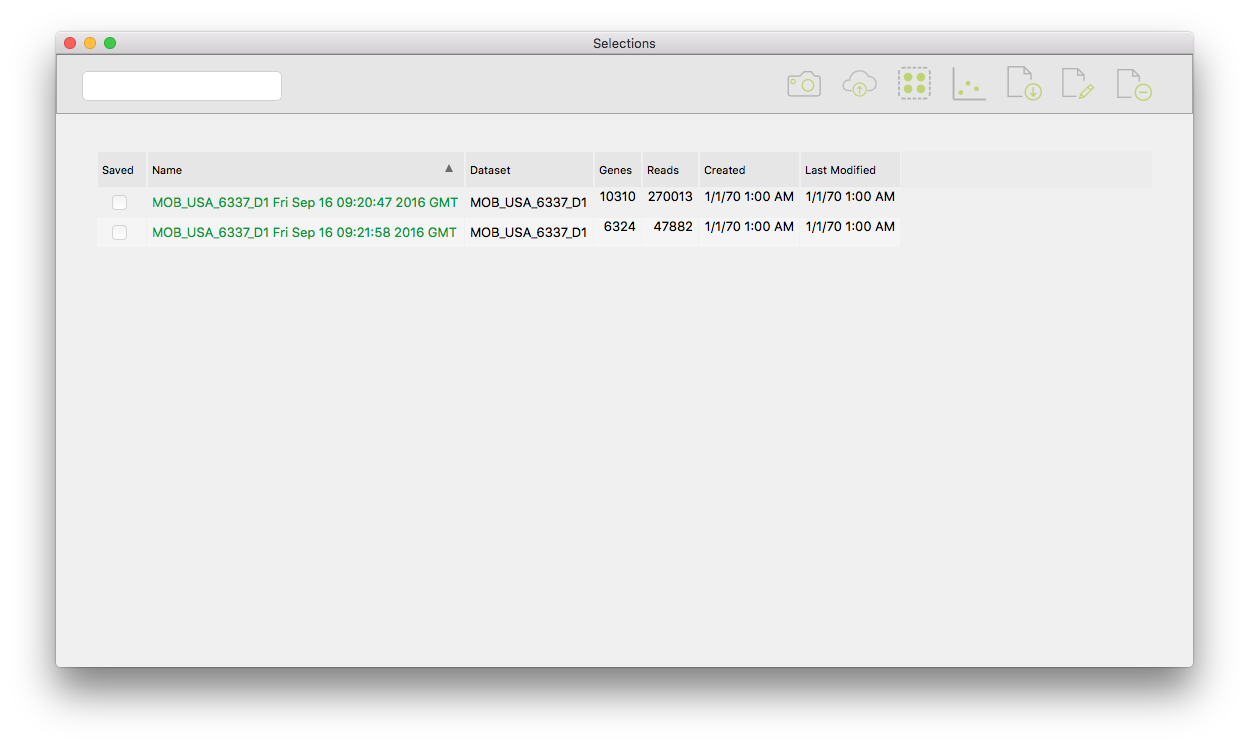
\includegraphics[width=0.8\linewidth]{./Pictures/selection_menu}
	\caption{The selection window.}
	\label{fig:selection_menu}
\end{figure}

The selection menu lists all the selections that have been made in the current sample. The textbox on the top left enables the user to narrow down the list of selections. The buttons on the right, in order, show an image of the visual canvas with the selection that was used, saves the current selection to the cloud, shows the list of genes in the selection (along with the count of genes, figure \ref{fig:selection_gene_list}), performs a differential expression analysis on the selected selections (figure \ref{fig:de}), saves the current selection to the local computer, edits the name and details of the current selection, and remove the current selection. Selections are saved as tab separated text files. The show snapshot option shows a screenshot of the image when the selection was made. This is useful if the image was zoomed or panned to show a specific area.

When running in online mode, selectiond can be saved to the cloud and previously saved selections are shown and can be re-selected.

\begin{figure}[h]
	\centering
	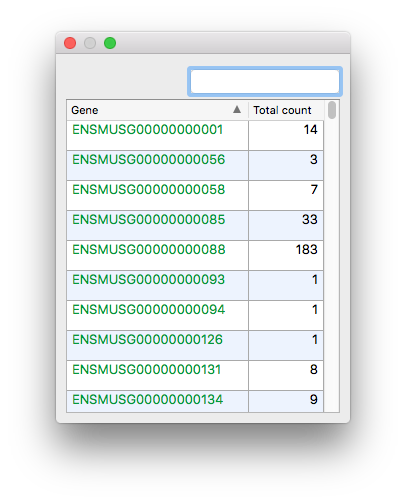
\includegraphics[scale=0.5]{./Pictures/selection_gene_list}
	\caption{The genes in the current selection.}
	\label{fig:selection_gene_list}
\end{figure}

\clearpage

\section{Differential Expression Window}

The differential expression window shows a log-log graph of counts for each gene in both selections, a list of all the genes and their counts in both selections and some statistics for the differential expression analysis. The statistics include The number of genes in both selections, the number of genes present in both selections, and the number of genes unique to each selection. Also displayed is the Pearson correlation for the differential expression. It is also possible to change the threshold for the number of reads used in the differential expression analysis. Changing the threshold changes both what is displayed on the graph, and also recomputes the Pearson correlation. The save button will save the current graph to the local computer.

\begin{figure}[h]
	\centering
	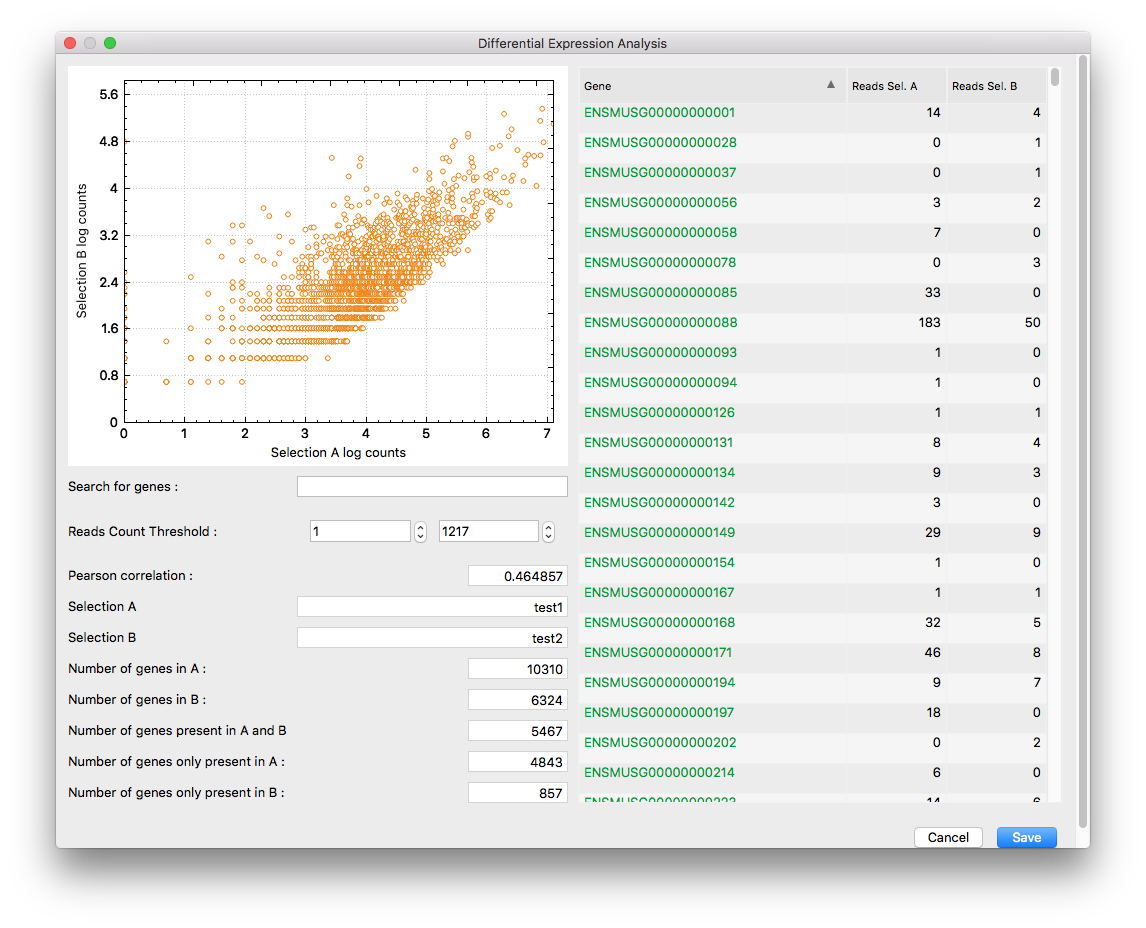
\includegraphics[width=0.8\linewidth]{./Pictures/DE_view}
	\caption[The differential expression window.]{The differential expression window.}
	\label{fig:de}
\end{figure}

\chapter{Known Issues and Future Plans}
\section{Known Issues}

As the application is still in the early alpha phase it may contain functional as well as visual discrepancies and issues. Some of these are known but were out of the scope of this release.

Below follows a list detailing each known issue, the afflicted platform as well as a brief description of its effect:

\begin{itemize}
\item	General
\subitem		Speed and memory issues
\item	Linux
\subitem		Some GUI related artifacts
\item	Windows
\subitem		Some GUI related artifacts
\end{itemize}

%\section{Future Plans}

\begin{appendices}
\chapter*{Appendix A - Installing the viewer}\label{Appendix A}
\addcontentsline{toc}{chapter}{Appendix A}
\section*{Installing in OSX}
\addcontentsline{toc}{section}{Installing in OSX}

\begin{itemize}[itemsep=10pt]
\item Download and install Qt from: \url{http://qt-project.org/downloads}
\item Download and extract QCustomplot sources from \url{http://qcustomplot.com/}
\item Install the necessary dependencies by running the following code (assuming MacPorts is installed)
\begin{verbatim}
sudo port install xcode cmake git
\end{verbatim}
NOTE: Make sure the XCode command line tools are installed.
\item Clone the repository and build the application. Remember to tell CMake where QCustomplot is using \texttt{DCMAKE\_PREFIX\_PATH}.
\vspace{1pt}
\begin{verbatim}
git clone https://github.com/SpatialTranscriptomicsResearch/st_viewer /path/to/source
mkdir /path/to/build
cd /path/to/build
cmake   [-DCMAKE_INSTALL_PREFIX="/usr/local/bin"] \
        [-DCMAKE_BUILD_TYPE="Debug | Release"] \
        [-DCMAKE_PREFIX_PATH="/path/to/libraries"] \
        [-DCMAKE_OSX_SYSROOT="/path/to/macosx.sdk"] \
        [-DCMAKE_OSX_DEPLOYMENT_TARGET=version] \
        [-DPUBLICKEY="path_to_ssl_key"] \
        [-DCONFIG_FILE="path/to/network_config_file"]
        /path/to/source
\end{verbatim}
\vspace{10pt}
\begin{itemize}
\item[] Where:
\item[] \texttt{DCMAKE\_INSTALL\_PREFIX} is where to install the viewer.
\item[] \texttt{DCMAKE\_BUILD\_TYPE} indicates the type of build (Debug or Release, default is Release).
\item[] \texttt{DCMAKE\_PREFIX\_PATH} is the location of any extra files (e.g. binaries for Qt5 and the source for QCustomplot).
\item[] \texttt{DCMAKE\_OSX\_SYSROOT} is the path to the MacOSX SDK that is to be used (e.g. \texttt{/Applications/Xcode.app/Contents/Developer/Platforms/MacOSX.platform/Developer/SDKs/MacOSX10.9.sdk/}.
\item[] \texttt{DCMAKE\_OSX\_DEPLOYMENT\_TARGET} is the target OSX version (can be older than the version of OSX running on the computer).
\item[] \texttt{DPUBLIC\_KEY} [optional] is the public key to access datasets in the online database.
\item[] \texttt{DCONFIG\_FILE} [optional] is the config file that is needed to access datasets in the online database. This file contains the endpoints and OAuth access settings. This file is loaded at runtime and is able to be edited after the viewer is installed.
\end{itemize}
\item Build the application.
\begin{verbatim}
make -j8
\end{verbatim}
\item Alternatively, you can build a standalone DMG bundle that you can install and/or distribute.
\begin{verbatim}
make dmg
\end{verbatim}
\end{itemize}

\pagebreak
\section*{Installing in UNIX}
\addcontentsline{toc}{section}{Installing in UNIX}

\begin{itemize}[itemsep=10pt]
\item Download and install Qt from: \url{http://qt-project.org/downloads}
\item Download and extract QCustomplot sources from \url{http://qcustomplot.com/}
\item Open a terminal and issue the following commands (apt-get in Ubuntu, yum in Fedora etc.)
\begin{verbatim}
sudo apt-get install cmake git ubuntu-dev-tools
sudo apt-get install libglu1-mesa-dev freeglut3-dev mesa-common-dev
\end{verbatim}
\item Clone the repository and build the application. Remember to tell CMake where QCustomplot is using \texttt{DCMAKE\_PREFIX\_PATH}.
\vspace{1pt}
\begin{verbatim}
git clone https://github.com/SpatialTranscriptomicsResearch/st_viewer /path/to/source
mkdir /path/to/build
cd /path/to/build
cmake   [-DCMAKE_INSTALL_PREFIX="/usr/local/bin"] \
        [-DCMAKE_BUILD_TYPE="Debug | Release"] \
        [-DCMAKE_PREFIX_PATH="/path/to/libraries"] \
        [-DCMAKE_OSX_SYSROOT="/path/to/macosx.sdk"] \
        [-DCMAKE_OSX_DEPLOYMENT_TARGET=version] \
        [-DPUBLICKEY="path_to_ssl_key"] \
        [-DCONFIG_FILE="path/to/network_config_file"]
        /path/to/source
\end{verbatim}
\vspace{10pt}
\begin{itemize}
\item[] Where:
\item[] \texttt{DCMAKE\_INSTALL\_PREFIX} is where to install the viewer.
\item[] \texttt{DCMAKE\_BUILD\_TYPE} indicates the type of build (Debug or Release, default is Release).
\item[] \texttt{DCMAKE\_PREFIX\_PATH} is the location of any extra files (e.g. binaries for Qt5 and the source for QCustomplot).
\item[] \texttt{DCMAKE\_OSX\_SYSROOT} is the path to the MacOSX SDK that is to be used (e.g. \texttt{/Applications/Xcode.app/Contents/Developer/Platforms/MacOSX.platform/Developer/SDKs/MacOSX10.9.sdk/}.
\item[] \texttt{DCMAKE\_OSX\_DEPLOYMENT\_TARGET} is the target OSX version (can be older than the version of OSX running on the computer).
\item[] \texttt{DPUBLIC\_KEY} [optional] is the public key to access datasets in the online database.
\item[] \texttt{DCONFIG\_FILE} [optional] is the config file that is needed to access datasets in the online database. This file contains the endpoints and OAuth access settings. This file is loaded at runtime and is able to be edited after the viewer is installed.
\end{itemize}
\item Issue the following commands to build and install the viewer.
\begin{verbatim}
make -j8
make install
\end{verbatim}
\item To build a standalone package to install and/or distribute:
\begin{verbatim}
make package
\end{verbatim}
\end{itemize}

\pagebreak
\section*{Installing in Windows}
\addcontentsline{toc}{section}{Installing in Windows}
There are many different ways to build the ST Viewer in Windows. Here Cygwin is used.
\end{appendices}

\end{document}
